\chapter{Introduction to ICMP}
\minitoc

\newpage
\section{What is ICMP?}
ICMP (Internet Control Message Protocol) is a network layer protocol used for error reporting and diagnostic purposes in IP networks. It helps devices communicate issues like unreachable hosts or network congestion.

\section{Why is ICMP Important?}
ICMP is important because it enables network devices to report errors, diagnose issues, and manage communication. It supports tools like \texttt{ping} and \texttt{traceroute}, which are essential for troubleshooting and maintaining network health.

Here are some use cases for ICMP:
\subsection{Error reporting}
ICMP error messages report networking errors, such as unreachable destinations, timeouts, or fragmentation problems. The messages are especially important for User Datagram Protocol (UDP), which has a connectionless communications model.

UDP does not provide reliable, ordered delivery of packets. When a UDP packet is sent, it’s possible that the packet may be lost, or it may be delivered with faults such as checksum errors. If this happens, the receiver sends ICMP error reporting messages back to the sender to notify it of the problem.

\subsection{Diagnostics}
You can use ICMP for network diagnostics. It’s most commonly used for ping and traceroute commands.

The ping command tests the reachability of network devices by sending ICMP echo request packets to a target device. If the device is reachable, it returns an ICMP echo reply. It reliably checks network latency and ensures the device is available.

The traceroute command traces the path taken by packets from a source to a destination. To do this, the command sends echo request and echo reply messages to the intended destination.

Echo requests contain a time-to-live (TTL) value, which decreases by one each time the packet passes through a router. When a packet reaches a router with a TTL of zero, the router sends an ICMP message back to the source.

The message contains information about the route taken by the packet. Traceroute reveals the exact path of a packet, which can provide you with network performance insights.

\subsection{Network security}
You can use ICMP to detect unauthorized network traffic and permit only legitimate traffic over a network. Firewalls use ICMP to allow or block certain types of traffic. Network administrators also use ICMP monitoring tools to track the status and connectivity of network devices and detect unknown devices.

You can also use it to spot unusual traffic patterns that may indicate unauthorized activity.

\section{How ICMP Fits into the TCP/IP and OSI Models}
ICMP operates at the Network Layer (Layer 3) in the OSI models. In the TCP/IP model, it is part of the Internet Layer (Layer 2), ICMP works alongside IP to provide error reporting and diagnostic functions.

\noindent Figure \ref{fig:icmp_models} illustrates the position of ICMP in both the TCP/IP and OSI models.


\begin{figure}[h]
	\centering
	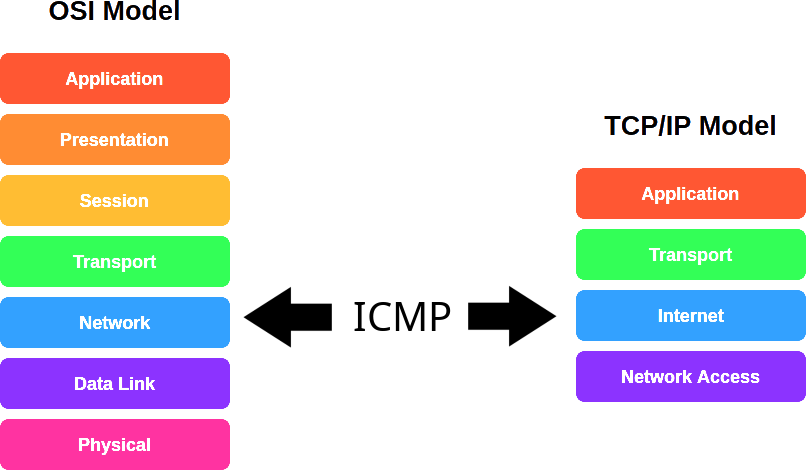
\includegraphics[width=1\textwidth]{assets/layers2.png}
	\caption{Position of ICMP in the TCP/IP and OSI Models}
	\label{fig:icmp_models}
\end{figure}

\newpage



 








